%%%%%%%%%%%%%%%%%%%%%%%%%%%%%%%%%%%%%%%%%
% Jacobs Landscape Poster
% LaTeX Template
% Version 1.1 (14/06/14)
%
% Created by:
% Computational Physics and Biophysics Group, Jacobs University
% https://teamwork.jacobs-university.de:8443/confluence/display/CoPandBiG/LaTeX+Poster
% 
% Further modified by:
% Nathaniel Johnston (nathaniel@njohnston.ca)
%
% This template has been downloaded from:
% http://www.LaTeXTemplates.com
%
% License:
% CC BY-NC-SA 3.0 (http://creativecommons.org/licenses/by-nc-sa/3.0/)
%
%%%%%%%%%%%%%%%%%%%%%%%%%%%%%%%%%%%%%%%%%

%----------------------------------------------------------------------------------------
%	PACKAGES AND OTHER DOCUMENT CONFIGURATIONS
%----------------------------------------------------------------------------------------

\documentclass[final]{beamer}

\usepackage[scale=1.24]{beamerposter} % Use the beamerposter package for laying out the poster

\usetheme{confposter} % Use the confposter theme supplied with this template

\setbeamercolor{block title}{fg=ngreen,bg=white} % Colors of the block titles
\setbeamercolor{block body}{fg=black,bg=white} % Colors of the body of blocks
\setbeamercolor{block alerted title}{fg=white,bg=dblue!70} % Colors of the highlighted block titles
\setbeamercolor{block alerted body}{fg=black,bg=dblue!10} % Colors of the body of highlighted blocks
% Many more colors are available for use in beamerthemeconfposter.sty

%-----------------------------------------------------------
% Define the column widths and overall poster size
% To set effective sepwid, onecolwid and twocolwid values, first choose how many columns you want and how much separation you want between columns
% In this template, the separation width chosen is 0.024 of the paper width and a 4-column layout
% onecolwid should therefore be (1-(# of columns+1)*sepwid)/# of columns e.g. (1-(4+1)*0.024)/4 = 0.22
% Set twocolwid to be (2*onecolwid)+sepwid = 0.464
% Set threecolwid to be (3*onecolwid)+2*sepwid = 0.708

\newlength{\sepwid}
\newlength{\onecolwid}
\newlength{\twocolwid}
\newlength{\threecolwid}
\setlength{\paperwidth}{48in} % A0 width: 46.8in
\setlength{\paperheight}{36in} % A0 height: 33.1in
\setlength{\sepwid}{0.024\paperwidth} % Separation width (white space) between columns
\setlength{\onecolwid}{0.22\paperwidth} % Width of one column
\setlength{\twocolwid}{0.464\paperwidth} % Width of two columns
\setlength{\threecolwid}{0.708\paperwidth} % Width of three columns
\setlength{\topmargin}{-0.5in} % Reduce the top margin size
%-----------------------------------------------------------

\usepackage{graphicx}  % Required for including images
\usepackage{tikz}						% To draw
\usetikzlibrary{shapes,snakes,arrows}				% Tikz shapes
\usepackage{booktabs} % Top and bottom rules for tables

\tikzstyle{block} = [draw, rectangle, minimum width = 0.75cm, minimum height = 0.75cm]
\tikzstyle{dot} = [draw, circle, minimum size=.5cm, node distance=1.75cm]

\newcommand{\bit}[0]{\begin{itemize}}
\newcommand{\eit}[0]{\end{itemize}}

\makeatletter							%This allows for a thicker hline in tabular
\newcommand{\thickhline}{%
    \noalign {\ifnum 0=`}\fi \hrule height 1pt
    \futurelet \reserved@a \@xhline
}
\makeatother

%----------------------------------------------------------------------------------------
%	TITLE SECTION 
%----------------------------------------------------------------------------------------

\title{From Latin to Romance: Computational Modeling of Syncretism} % Poster title

\author{Tyler Lau$^*$, Maria Polinsky$^\dagger$, and Jake Seaton$^\dagger$} % Author(s)

\institute{$^*$Department of Linguistics, University of California at Berkeley, USA \\
$^\dagger$Deparment of Linguistics, Harvard University, USA} % Institution(s)

%----------------------------------------------------------------------------------------

\begin{document}

\addtobeamertemplate{block end}{}{\vspace*{2ex}} % White space under blocks
\addtobeamertemplate{block alerted end}{}{\vspace*{2ex}} % White space under highlighted (alert) blocks

\setlength{\belowcaptionskip}{2ex} % White space under figures
\setlength\belowdisplayshortskip{2ex} % White space under equations

\begin{frame}[t] % The whole poster is enclosed in one beamer frame

\begin{columns}[t] % The whole poster consists of three major columns, the second of which is split into two columns twice - the [t] option aligns each column's content to the top

\begin{column}{\sepwid}\end{column} % Empty spacer column

\begin{column}{\onecolwid} % The first column

%----------------------------------------------------------------------------------------
%	OVERVIEW
%----------------------------------------------------------------------------------------

\begin{alertblock}{Overview}

\small\textbf{Questions:} 
\bit
	\item What factors in Late Latin led to the heavy reshaping of the nominal system?
	\item What minimal information does a connectionist model need to predict syncretism in the correct direction?
\eit
\textbf{Background:}
\bit
%	\item Paradigm leveling and analogical extension have been extensively described in the literature (CITE)
	\item Analogy driven by factors such as \textit{frequency}, \textit{markedness}, \textit{morpheme length}, etc. (Kurylowicz 1947, Manczak 1958, Bybee 1985, Hock 1991, Albright 2008)
	\item From Latin to Romance
	\bit
		\item Declension: 5 $>$ 3$\sim$2 (I, II, (III)): frequency, sound change
		\item Gender: 3 $>$ 2 (M, F): sound change, contact
		\item Case: 6 $>$ 2$\sim$1 (\textsc{acc, (nom/gen)}): sound change, periphrastic constructions (preposition+\textsc{acc})
	\eit
	\item Fate of the Neuter
	\bit
		\item N.SG ended in same endings as M.SG so many became M
		\item N.PL ended in {\sl -a} and as plural inanimates were seen as collectives, reinterpreted as F.SG: ex. Lat. \textit{folia} `leaves N.PL' $>$ Sp. \textit{hoja} `leaf F.SG' (Herman 1967)
		\item Romanian has an ambigeneric system
		\bit
			\item ``Neuter'' class takes M morphology in singular and F in plural
			\item Falls out from same principles as other Romance languages (with N.PL being reinterpreted as F.PL)
			\item Many M's migrate to N class via analogy (Lat. \textit{campus} $\sim$ \textit{campi} `field M' $>$ Rom. \textit{c\^imp} (M.SG) $\sim$ \textit{c\^impuri} (F.PL) , likely via \textit{tempus} $\sim$ \textit{tempora} `time N')
		\eit
	\eit
%	\item (CITE ALBRIGHT 2002) provides a {\sl deterministic} model of analogy in which a {\sl base form} is determined via a confidence measure arrived at via informativeness (how much of the remainder of a paradigm can be arrived at given a form's information) and frequency
\eit
\textbf{Objective:} To use a connectionist simulation of generational learning providing minimal phonological and semantic information and see whether the changes that are actually attested in Romance can be reproduced

% TO DO:
%	Figure out what forms end up being preserved
%	Figure out whether the nouns that migrated are the right ones
%	This predicts forms, but not necessarily *meaning*
%	Change neural net so that GEN node is gone after 

% (DISCUSSION SECTION: works well with Albright's model suggesting that frequency plays a large role, also works well in suggesting that synchronic effects lead to diachronic effects)

\end{alertblock}

%----------------------------------------------------------------------------------------
%	LATIN DECLENSION SYSTEM
%----------------------------------------------------------------------------------------

\begin{block}{Latin Declension System}

\begin{figure}[h]
	\footnotesize
	\begin{tabular}{ll| llllll}
				&	&	I		&	II		&	IIIa		&	IIIb		&	IV		&	V	\\ \thickhline
%		&Final			&	a-		&	o-		&	C-		&	i-		&	u-		&	e-	\\
		& Root		&	silv\textbf{a}-		&	ann\textbf{o}-	&	colo\textbf{r}-	&	ign\textbf{i}-		&	lac\textbf{u}-		&	fid\textbf{e}-	\\
		& Gloss		&	`forest'	&	`year'	&	`color'	&	`fire'		&	`lake'	&	`faith'	\\ \hline
		& Nom.	&	silv\textbf{a}		&	ann\textbf{us}&	color	&	ign\textbf{is}	&	lac\textbf{us} &	fid\textbf{\=es} \\
		Sg. & Gen.		&	silv\textbf{ae} 	&	ann\textbf{\=\i}&	col\=or\textbf{is}&	ign\textbf{is}	&	lac\textbf{\=us}&	fid\textbf{e\=\i} \\
		& Acc.		&	silv\textbf{am}	&	ann\textbf{um}&	col\=or\textbf{em}& ign\textbf{em}&	lac\textbf{um}&	fid\textbf{em}	\\  \hline
%		&Dat.		&	silv\textbf{ae}		&	ann\textbf{\=o}&	col\=or\textbf{\=\i}& ign\textbf{\=\i}&	lac\textbf{u\=\i} &	fide\textbf{i}	\\
%%		&			&				&			&				& 		&	lac\textbf{\=u} & \\
%		&Abl.		&	silv\textbf{\=a}	&	ann\textbf{\=o}&	col\=or\textbf{e}& ign\textbf{e}/&	lac\textbf{\=u}&	fid\textbf{\=e}	\\
%		&			&				&			&				&	ign\textbf{\=\i}	&	\\
%		&Voc.		&	silv\textbf{a}	&	ann\textbf{e}&	color	& ign\textbf{is}&	lac\textbf{us}&	fid\textbf{\=es}	\\ \hline
%		Pl.		&				&			&			&		&			&		\\
		& Nom.	&	silv\textbf{ae}		&	ann\textbf{\=\i}&	col\=or\textbf{\=es}& ign\textbf{\=es}&	lac\textbf{\=us}&	fid\textbf{\=es}		\\
		Pl. & Gen.		&	silv\textbf{\=arum} 	&	ann\textbf{\=orum}	&	col\=or\textbf{um}&ign\textbf{ium}& lac\textbf{\=um}&	fid\textbf{\=erum}\\
		& Acc.		&	silv\textbf{\=as}	&	ann\textbf{\=os}&	col\=or\textbf{\=es}&	ign\textbf{\=\i s}/&	lac\textbf{\=us}&	fid\textbf{\=es} \\
		&			&				&			&				&	ign\textbf{\=es}&		& \\		
%		&Dat.		&	silv\textbf{\=\i s}	&	ann\textbf{\=\i s}&	col\=or\textbf{ibus}& ign\textbf{ibus}&	lac\textbf{ubus}&	fid\textbf{\=ebus}	\\
%		&Abl.		&	silv\textbf{\=\i s}	&	ann\textbf{\=\i s}&	col\=or\textbf{ibus}& ign\textbf{ibus}&	lac\textbf{ubus}&	fid\textbf{\=ebus}\\
%		&Voc.		&	silv\textbf{ae}	&	ann\textbf{\=\i}&	col\=or\textbf{\=es}& ign\textbf{\=es}&	lac\textbf{\=us}&	fid\textbf{\=es}		
	\end{tabular}
	\caption{The Latin Declension Classes}
	\label{fig:latdec}
\end{figure}

\end{block}

%----------------------------------------------------------------------------------------

\end{column} % End of the first column

\begin{column}{\sepwid}\end{column} % Empty spacer column

\begin{column}{\twocolwid} % Begin a column which is two columns wide (column 2)

%----------------------------------------------------------------------------------------
%	MODEL
%----------------------------------------------------------------------------------------

\begin{block}{Structure of the Connectionist Model}

\begin{figure}[t]
\footnotesize
\begin{tikzpicture}
	\draw [help lines] (0,0) grid (5,5);
	\node[draw, align=center] (hidden)	[block] {\textbf{Hidden Layer (30 nodes)}};
	\node[draw, align=center] (-5,0)		[block] {Pre-Input};
\end{tikzpicture}
\end{figure}

%\begin{columns}[t,totalwidth=\twocolwid] % Split up the two columns wide column
%
%\begin{column}{0.23\paperwidth}\vspace{-.6in} % The first column within column 2 (column 2.1)
%
%		\begin{figure}
%			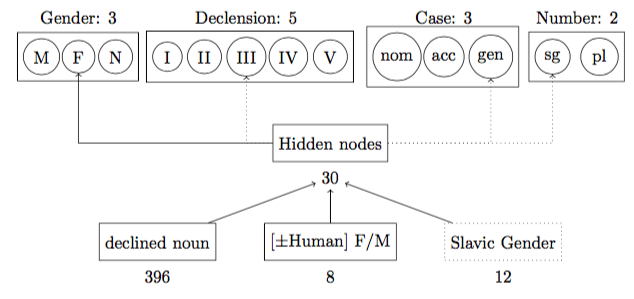
\includegraphics[height=.5\textwidth]{architecture.png}
%		\end{figure}
%
%%----------------------------------------------------------------------------------------
%
%\end{column} % End of column 2.1
%
%\begin{column}{0.25\paperwidth}\vspace{-.6in} % The second column within column 2 (column 2.2)
%
%\begin{figure}
%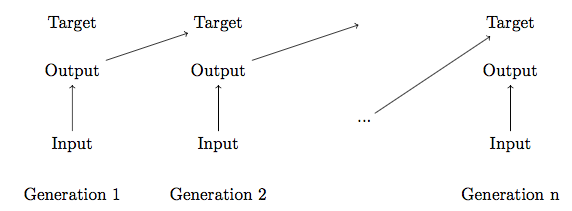
\includegraphics{generations.png}
%\end{figure}
%
%\end{column} % End of column 2.2
%
%\end{columns} % End of the split of column 2 - any content after this will now take up 2 columns width

\end{block}

%----------------------------------------------------------------------------------------
%	RESULTS
%----------------------------------------------------------------------------------------

\begin{block}{Results}

\begin{columns}[t]
      \begin{column}{.33\linewidth}
 \footnotesize
\begin{figure}
\begin{center} 
\vspace{2cm}
{\centering 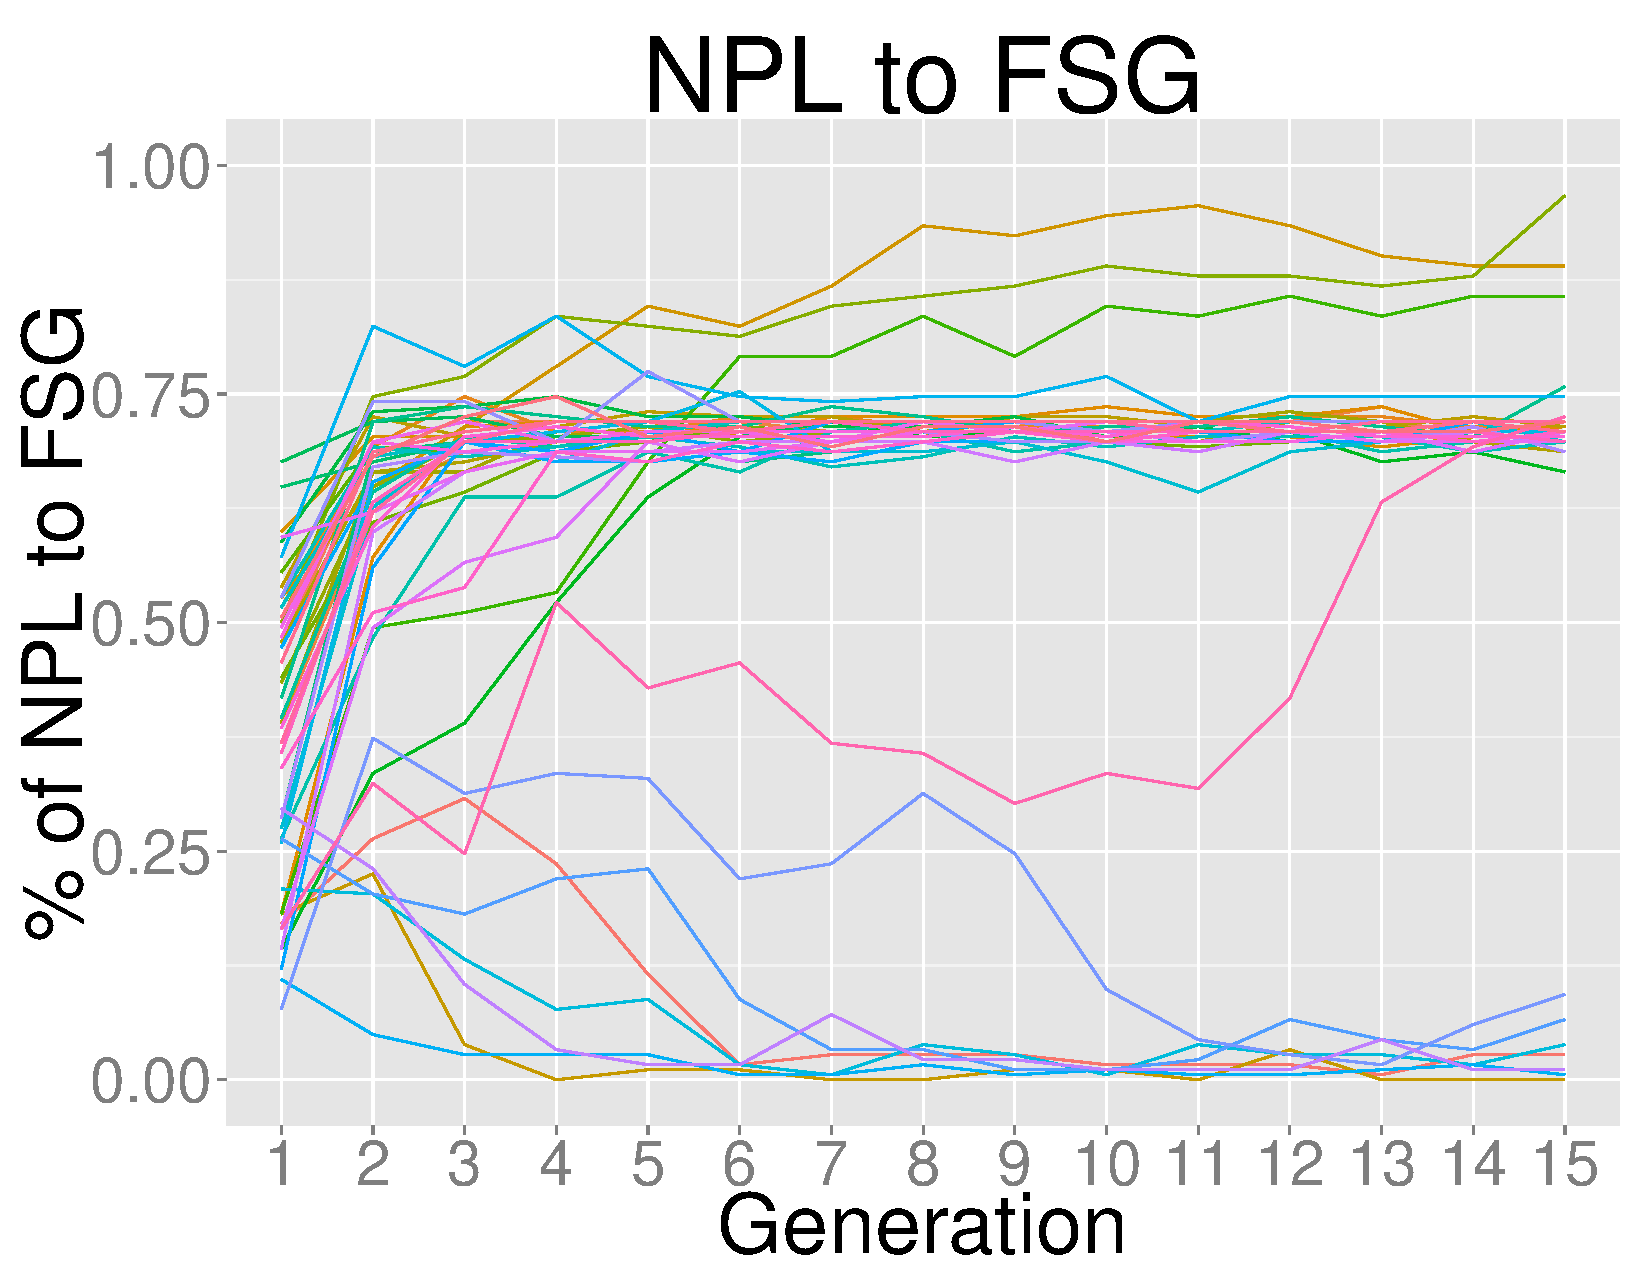
\includegraphics[width=1\textwidth]{npltofsg.pdf}}
\end{center}
\caption{\textit{With the genitive dropped, neuter plurals almost consistently migrate to the feminine singular class due to phonological similarity alone--while collective semantics can be invoked, they are not absolutely necessary to account for the facts.}}
\end{figure}    
      
      \end{column}
      
            \begin{column}{.33\linewidth}
            
\begin{figure}
\begin{center} 
\vspace{2cm}
{\centering 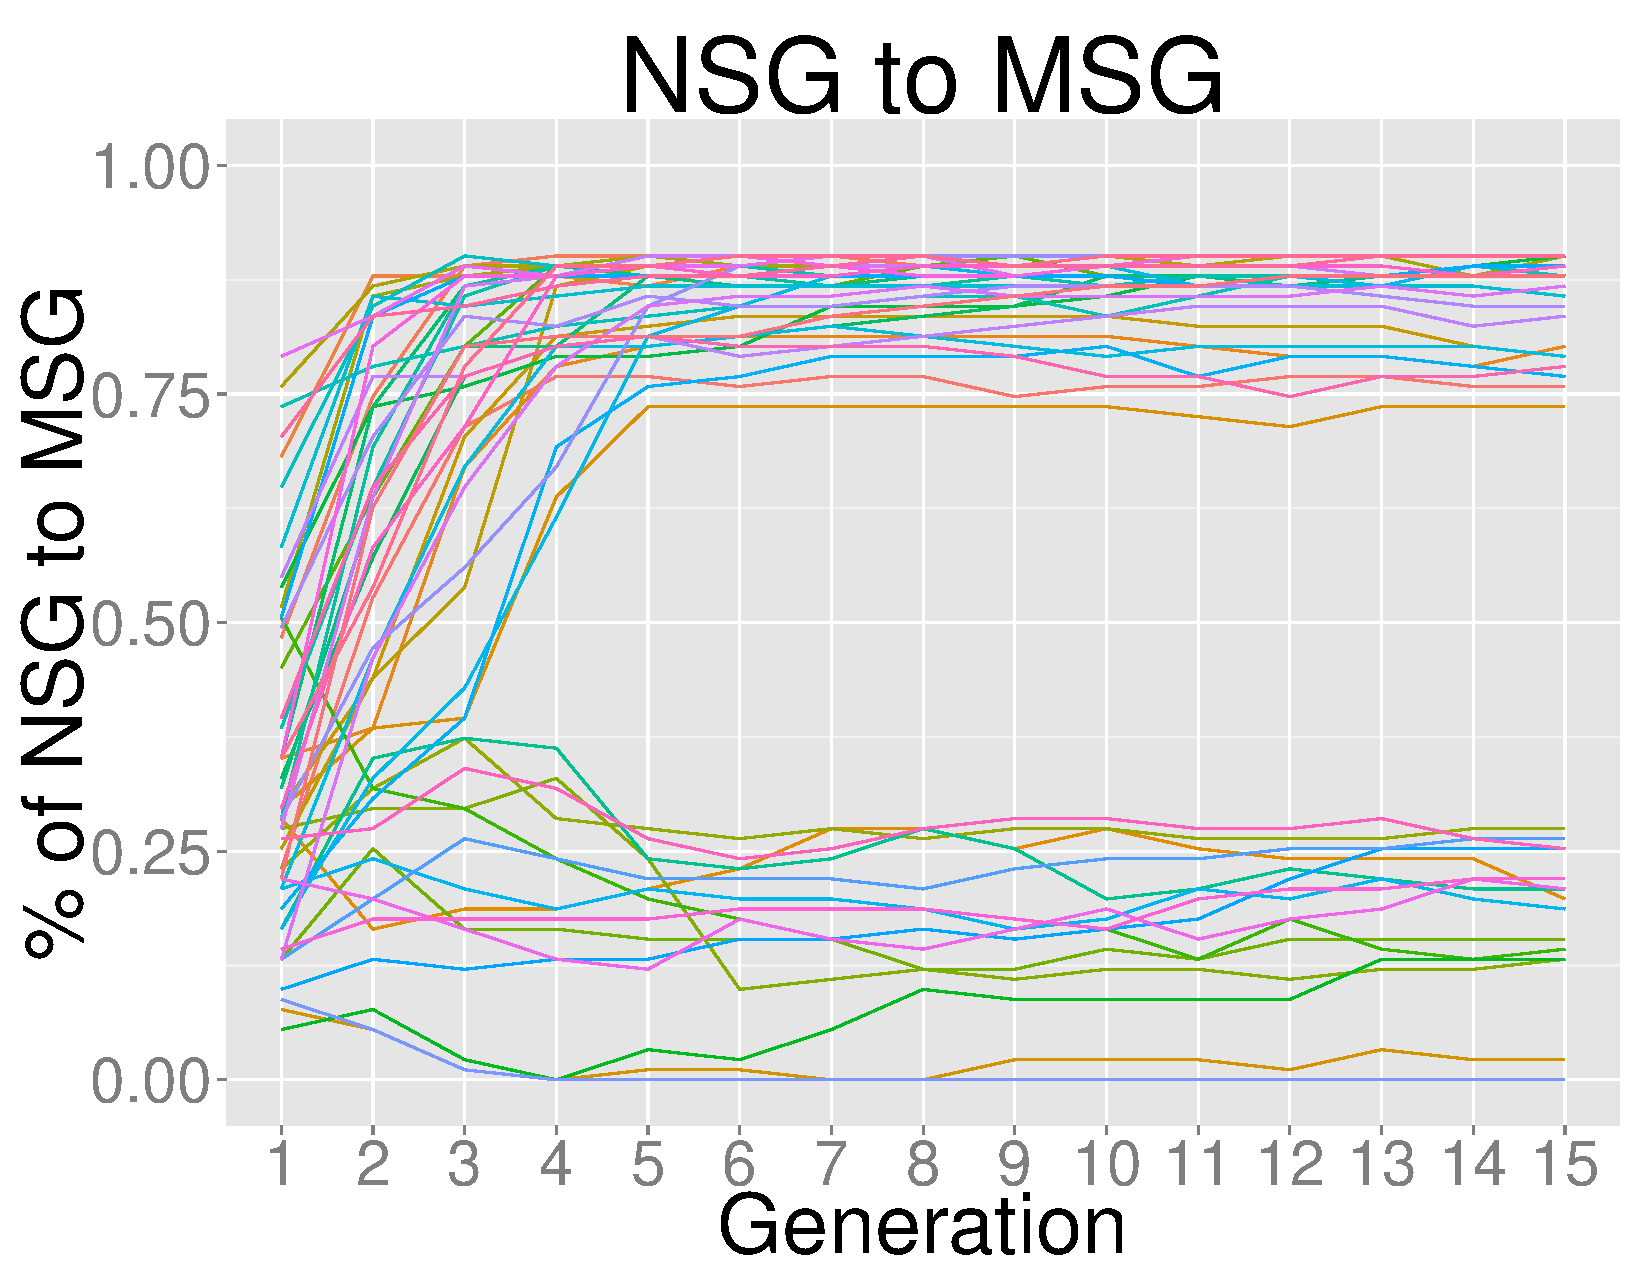
\includegraphics[width=1\textwidth]{nsgtomsg.pdf}}
\end{center}
\footnotesize
\caption{\textit{With the genitive dropped, neuter singulars undergo a bifurcation--they either merge almost completely with masculines or stay very much neuter while drawing masculines to their class (see Figure \ref{gendist}).}}
\end{figure}     
            
      \end{column}      
       \begin{column}{.33\linewidth}
\footnotesize
\begin{figure}
\begin{center} 
\vspace{2cm}
{\centering 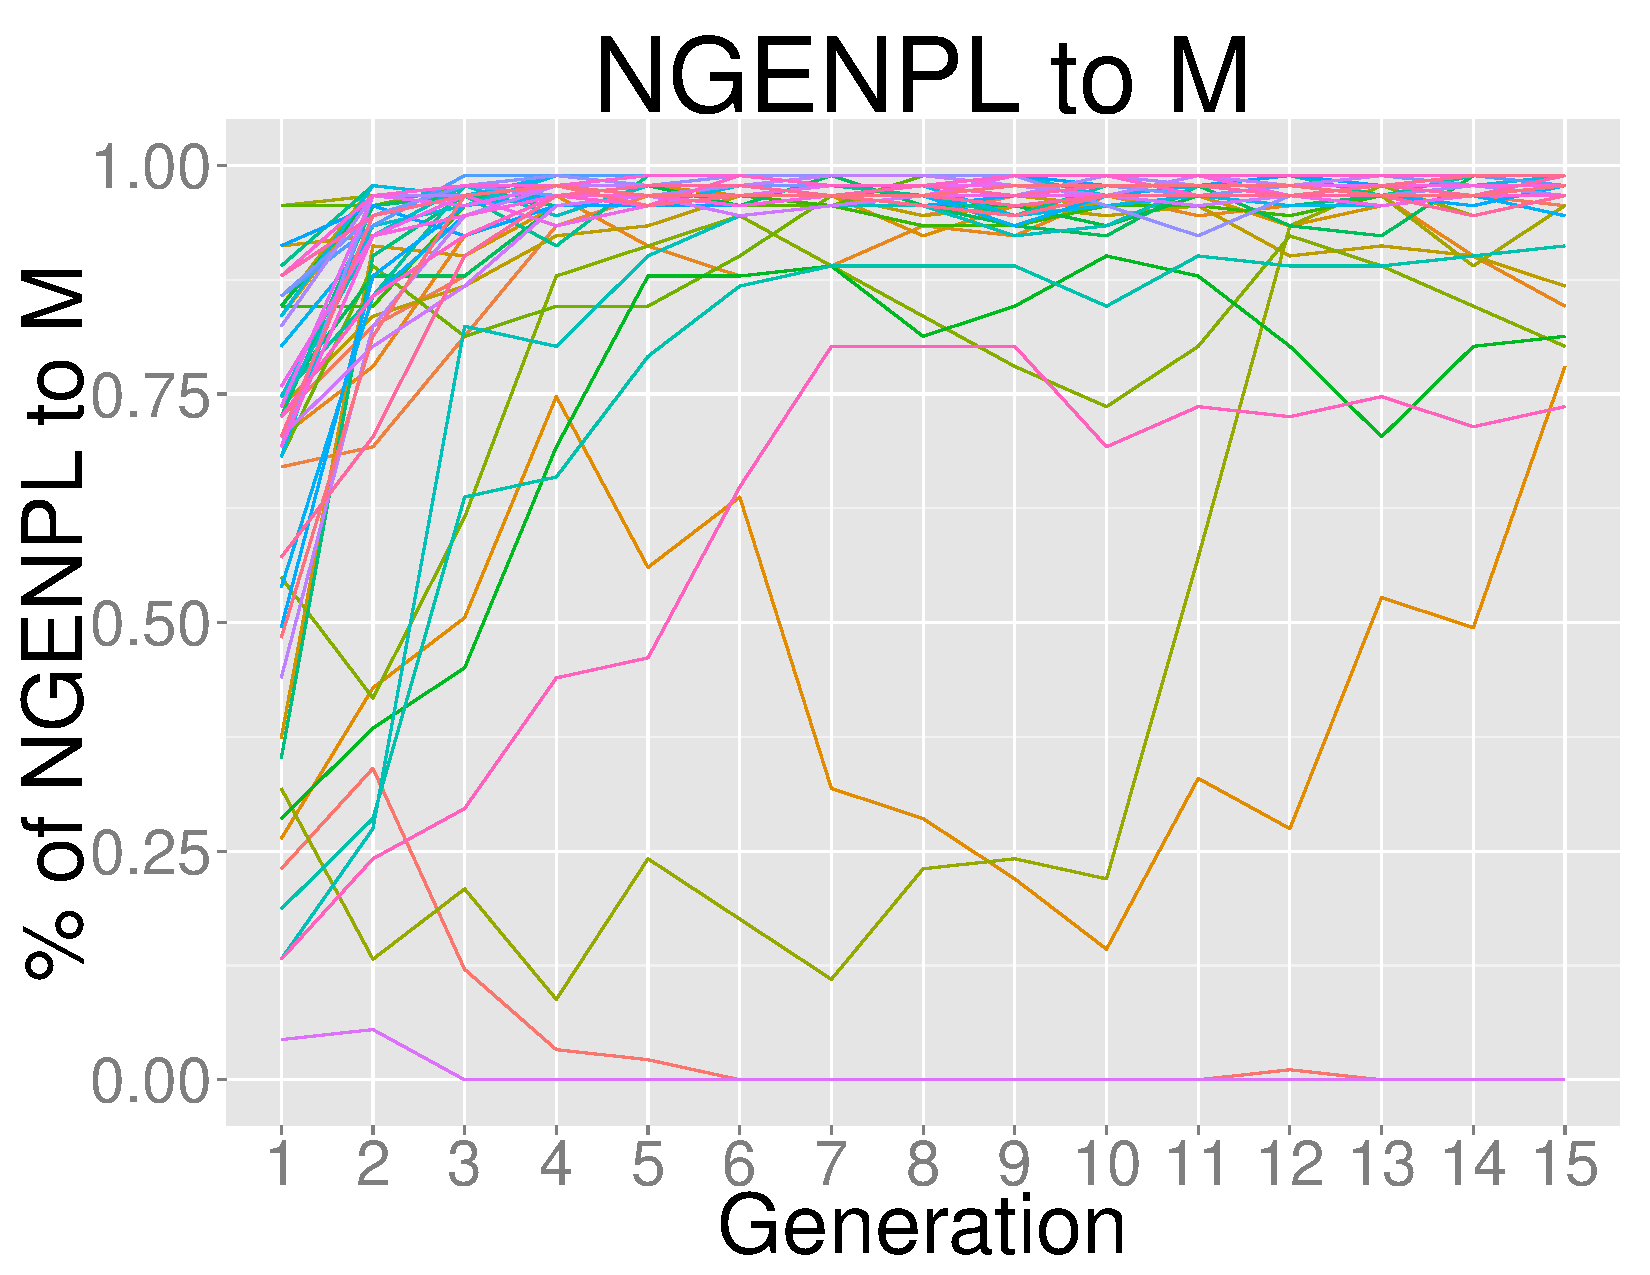
\includegraphics[width=1\textwidth]{ngenpltom.pdf}}
\end{center}
\caption{\textit{Without the genitive dropped, the genitive plurals are largely drawn to the masculine, as they do {\sl not} end in {\sl -a}. This prevents the neuter plurals from migrating almost categorically to F.SG.}}
\end{figure}           
       
      \end{column}    
    \end{columns}
    
\begin{columns}[t]
    \begin{column}{.33\linewidth}
    \begin{figure}
    \begin{center} 
	\vspace{2cm}
	{\centering 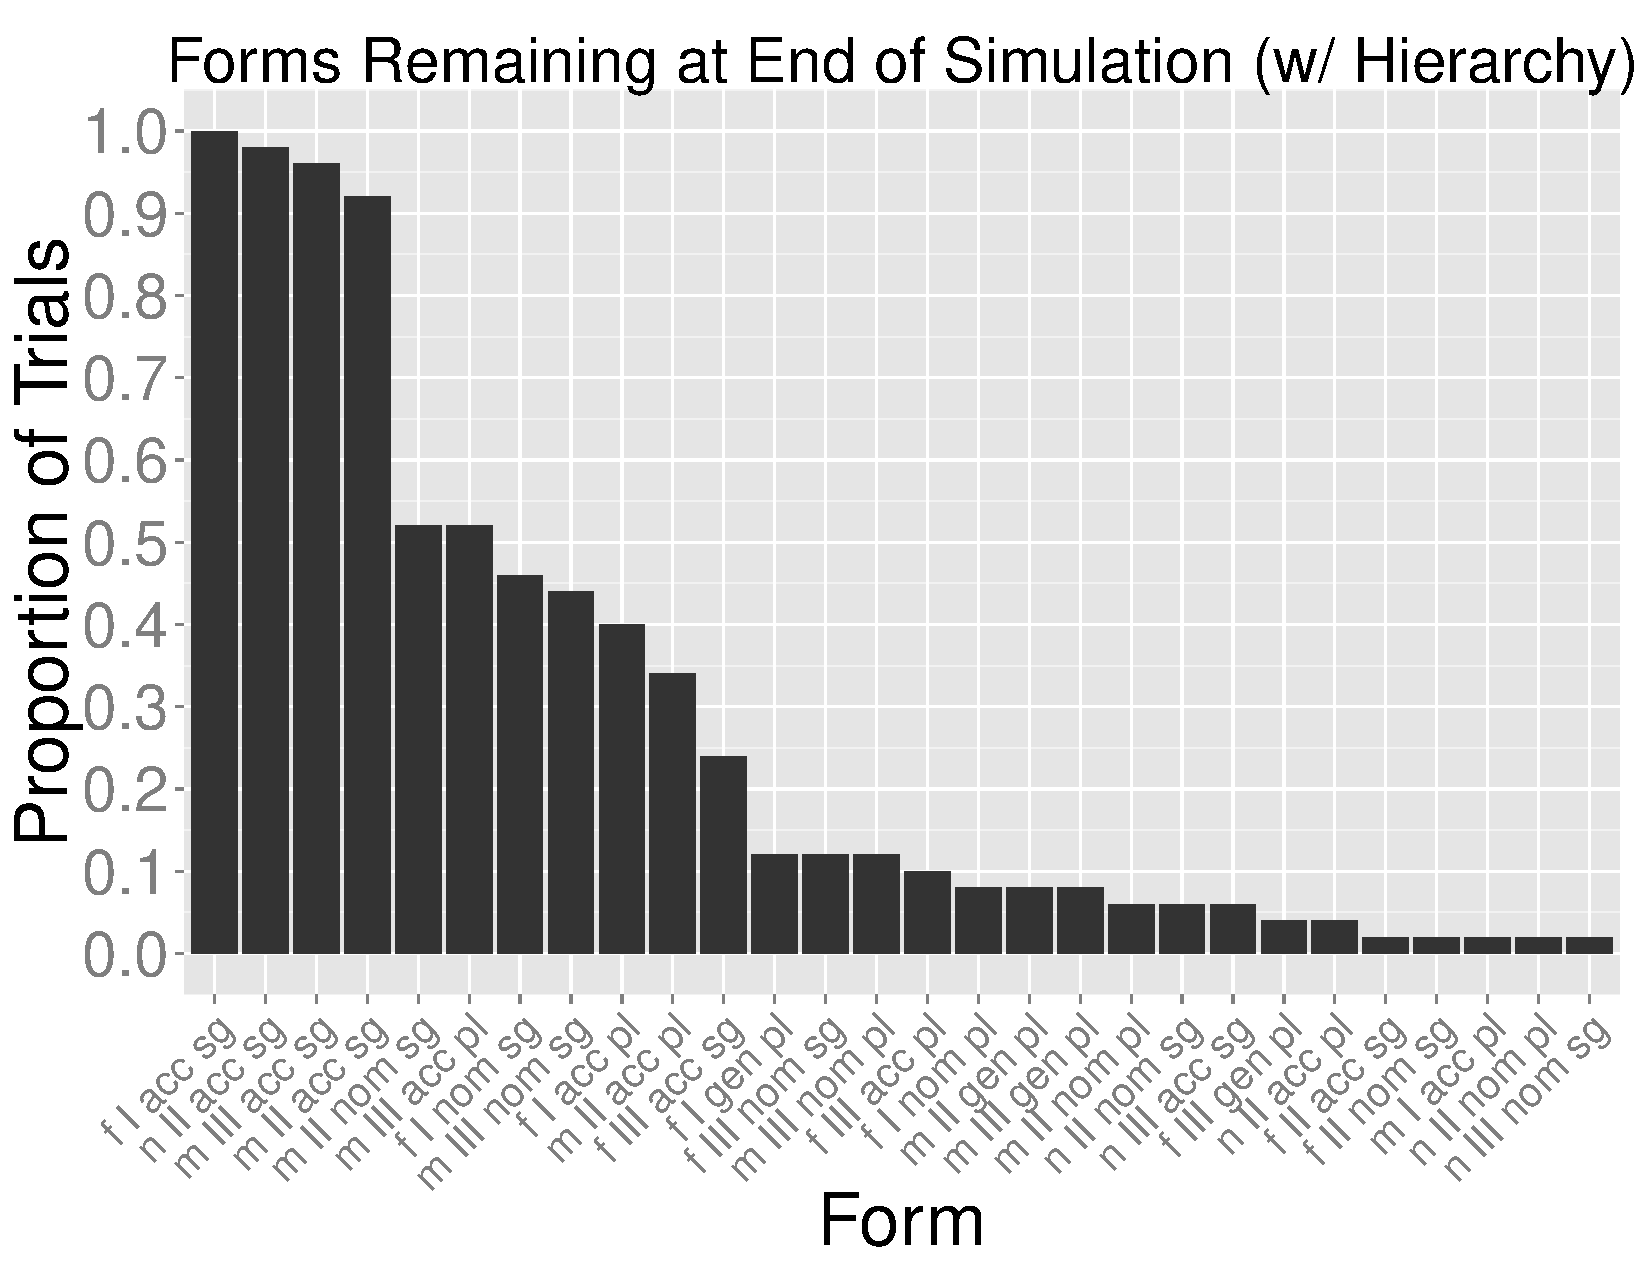
\includegraphics[width=1\textwidth]{endforms_hierarchy.pdf}}
	 \footnotesize
	\caption{\textit{With case hierarchy in play, the accusative is very robust, the genitive singular falls out completely, and the genitive plural survives in few cases. The most robust forms accord with history.}}
	\end{center}
	\end{figure}
    \end{column}
    
      \begin{column}{.33\linewidth}
      
      \begin{figure}
    \begin{center} 
	\vspace{2cm}
	{\centering 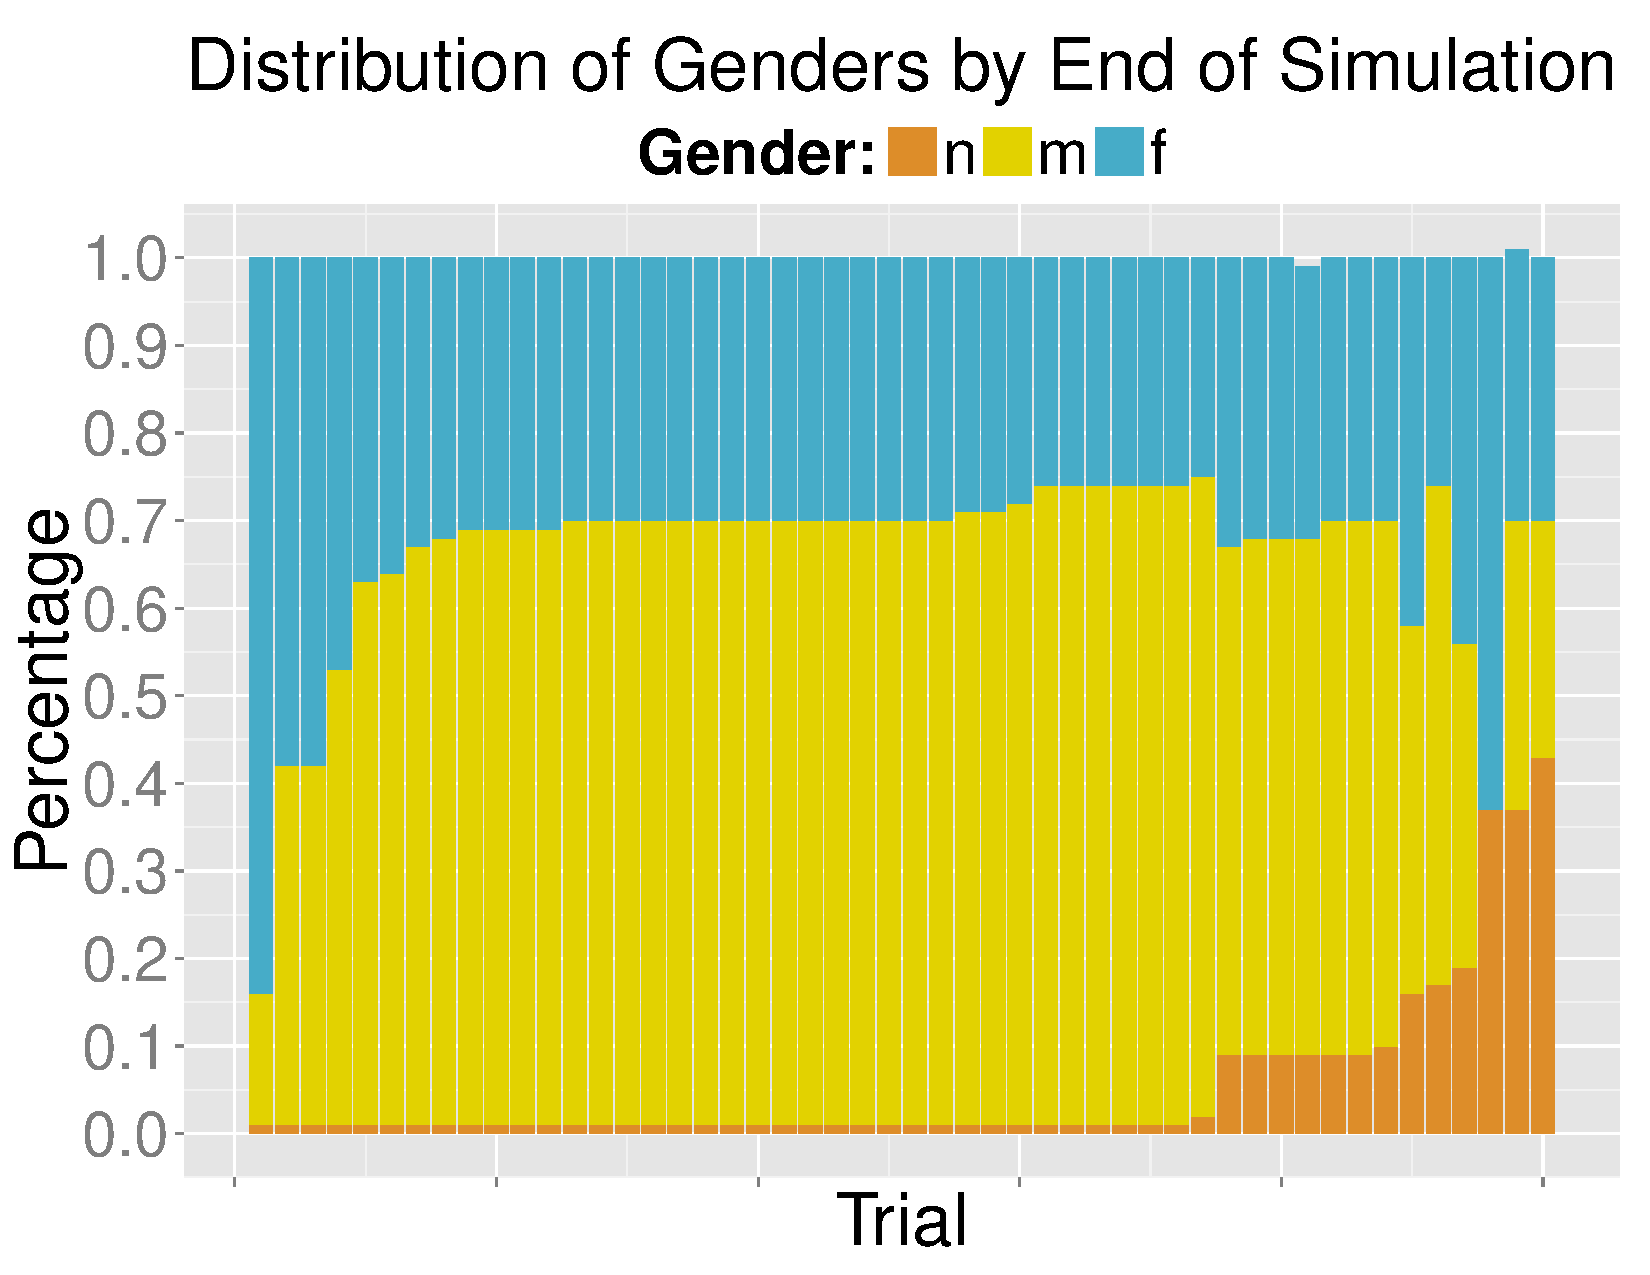
\includegraphics[width=1\textwidth]{genderdistribution.pdf}}
	\end{center}
	 \footnotesize
	\caption{\textit{In most of the trials, the neuter survives in at most a few words (this occurs in Italian, for example (\textit{dito} M.SG $\sim$ \textit{dita} F.PL `finger'). In the cases where it is more robust, M nouns migrate to the N class, as happened in Romanian.}}
	\label{gendist}
	\end{figure}
    \end{column}
 
      \begin{column}{.33\linewidth}
 	
    \begin{figure}
    \begin{center} 
	\vspace{2cm}
	{\centering 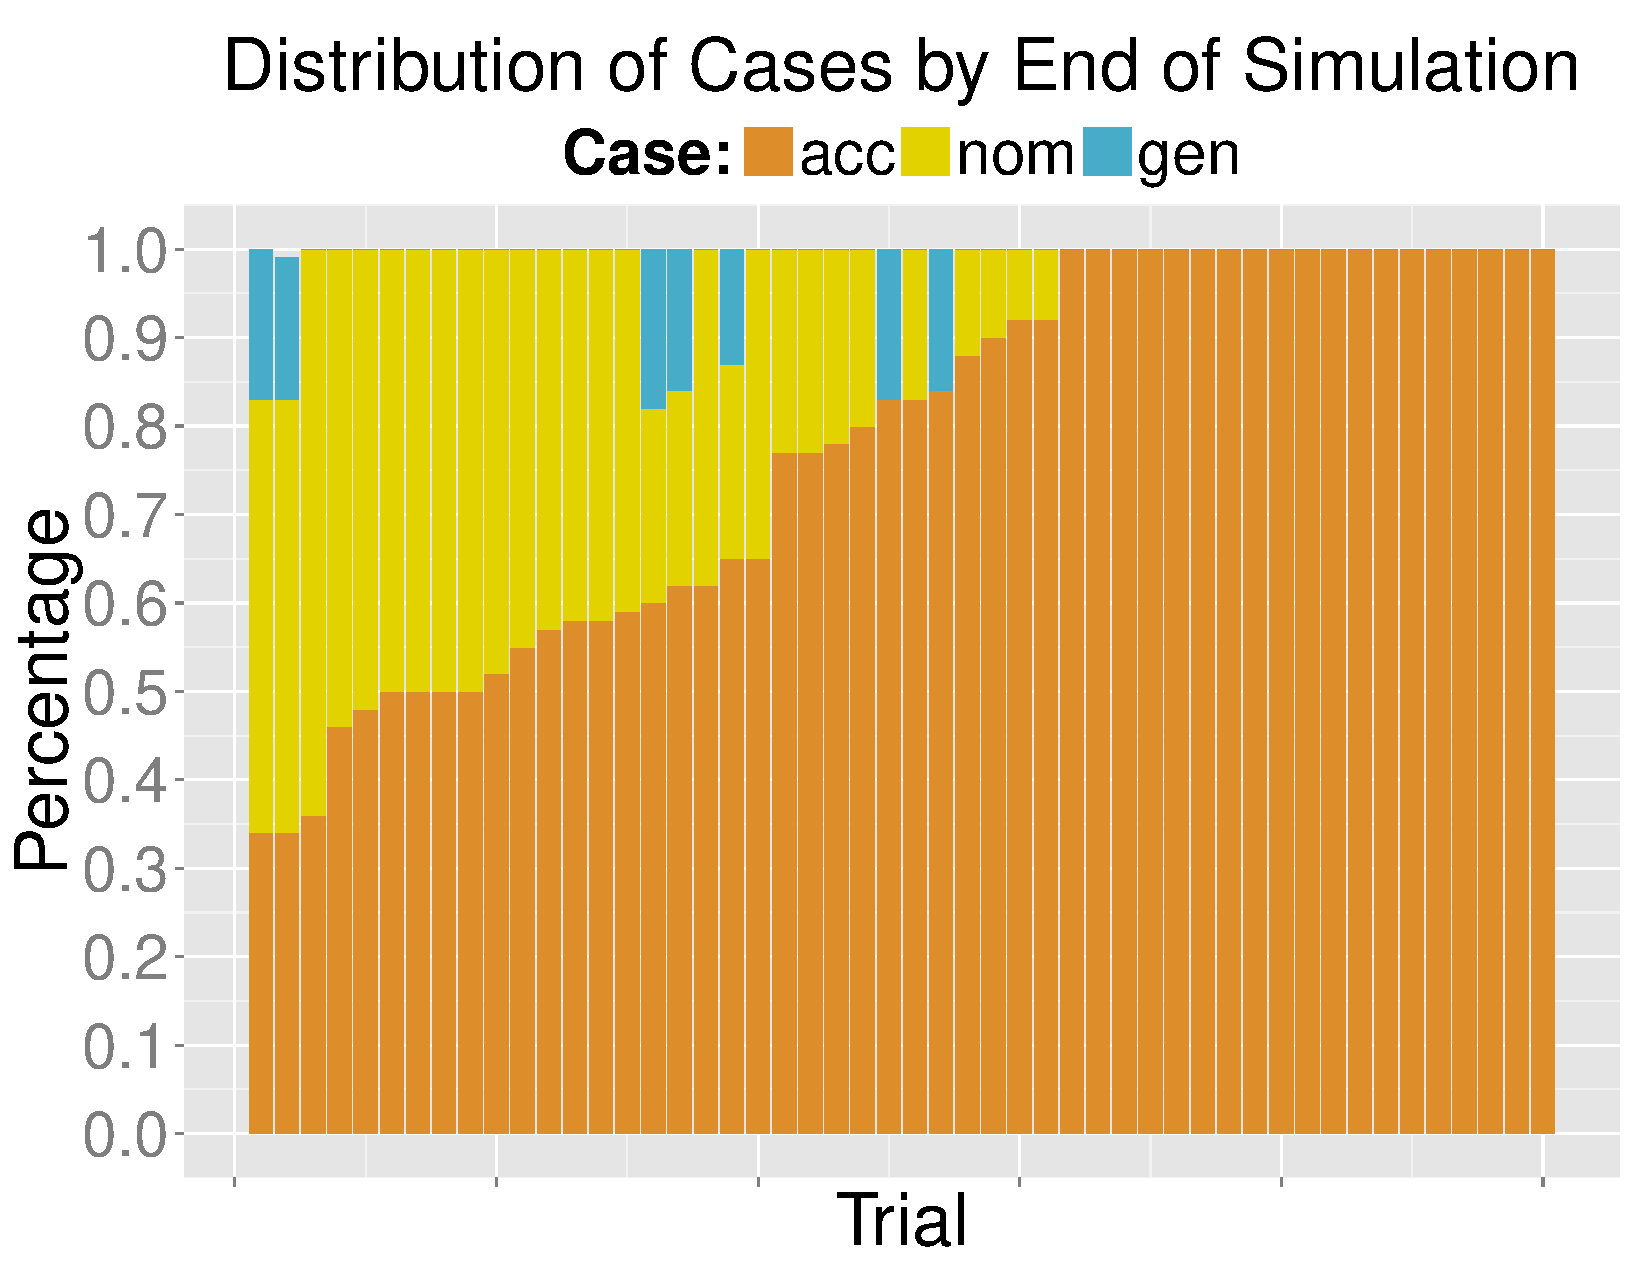
\includegraphics[width=1\textwidth]{casedistribution.pdf}}
	\end{center}
	 \footnotesize
	\caption{\textit{With case hierarchy in play, the accusative becomes the dominant case in almost every simulation and the only case in almost half. The genitive survives in hardly more than 10\% of trials}}
	\end{figure}
	
    \end{column}
\end{columns}

\end{block}

%----------------------------------------------------------------------------------------

\end{column} % End of the third column

\begin{column}{\sepwid}\end{column} % Empty spacer column

\begin{column}{\onecolwid} % The third column

%----------------------------------------------------------------------------------------
%	DISCUSSION
%----------------------------------------------------------------------------------------

\begin{alertblock}{Discussion}

\small
\bit
	\item With \textit{phonology}, \textit{frequency}, \& \textit{animacy semantics}
	\bit
		\item Declensions IV \& V fall out in \textit{every} simulation
	\eit
	\item With \textit{case hierarchy} added, final forms converge more
	\bit
		\item Genitive singular drops out \textit{completely}
		\item Genitive plural hardly survives (only example is oblique 3PL pronoun--Fr. \textit{leur}, It. \textit{loro}, Rom. \textit{lor})
		\item Forms remaining in $\geq$90\% of simulations
		\bit
			\item \textit{-am} $>$ \textit{-a} F.SG ending in all Romance ($>$ -\textit{e} in Fr.)
			\item \textit{-um} $>$ \textit{-u} M.SG ending in all of Romance ($>$ \textit{-o} in Sp., It. etc.)
			\item \textit{-em} $>$ \textit{-e} SG ending for M/F nouns in all of Romance
		\eit
		\item Forms remaining in 25-90\% of simulations
		\bit
			\item -$\varnothing$ SG ending for M/F nouns in all of Romance
			\item \textit{-\=es} PL ending in western Romance, maybe $>$ \textit{-i} in eastern
			\item \textit{-\=os} M.PL ending in western Romance, maybe $>$ \textit{-i} in eastern
			\item \textit{-\=as} F.PL ending in western Romance, maybe $>$ \textit{-e} in eastern
			\item M/F.NOM.SG \textit{-us} \& \textit{-as}: in E-Romance., final \textit{-s} falls out; in W-Romance, \textsc{nom} persists in older Sp. \& Fr.
		\eit
		\item Case system converges to accusative in almost half (as in western Romance), eastern Romance shows alternate history where nominative plural may have survived (see D'hulst (2005) on Romance plurals)
		\item Neuter rarely survives--when it stays, a sizeable chunk of the masculine class migrates over (as in Romanian)
	\eit
	\item With \textit{genitive} dropped, N.SG $>$ M.SG, N.PL $>$ F.SG
	\bit
		\item Otherwise, N.PL \textsc{gen} $>$ M.PL because of phonology
		\item Supports popularity of periphrastic construction view
	\eit
\eit

\end{alertblock}

%----------------------------------------------------------------------------------------
%	REFERENCES
%----------------------------------------------------------------------------------------

%\begin{block}{References}
%
%%\nocite{*} % Insert publications even if they are not cited in the poster
%\small{\bibliographystyle{li}
%\bibliography{tyler}\vspace{0.75in}}
%
%\end{block}

%----------------------------------------------------------------------------------------
%	ACKNOWLEDGEMENTS
%----------------------------------------------------------------------------------------

\setbeamercolor{block title}{fg=red,bg=white} % Change the block title color

\begin{block}{Acknowledgements}

\footnotesize{\rmfamily{Many thanks to Kevin Ryan, James Kirby, Andrew Garrett, Terry Regier, Mairi McLaughlin, and Yang Xu for comments and guidance throughout the project, to Ezra Van Everbroeck for providing the code for the simulation in Polinsky and Van Everbroeck (2003), and to Edwin Ko for consultation on data visualization. 
%Thanks as well to Teodora Mihoc, a native speaker of Romanian, who aided with Romanian data and to Marek Majer, who consulted on Proto-Slavic forms.
}} \\

\end{block}

%----------------------------------------------------------------------------------------
%	CONTACT INFORMATION
%----------------------------------------------------------------------------------------

\setbeamercolor{block alerted title}{fg=black,bg=norange} % Change the alert block title colors
\setbeamercolor{block alerted body}{fg=black,bg=white} % Change the alert block body colors

\begin{alertblock}{Contact Information}

\footnotesize

\begin{itemize}
\item Tyler Lau: \href{mailto:tylerlau@berkeley.edu}{tylerlau@berkeley.edu}
\item Maria Polinsky: \href{mailto:polinsky@fas.harvard.edu}{polinsky@fas.harvard.edu}
\item Jake Seaton: \href{mailto:jseaton@college.harvard.edu}{jseaton@college.harvard.edu}
\end{itemize}

\end{alertblock}

\begin{center}
\begin{tabular}{ccc}

\includegraphics[width=0.3\linewidth]{UC_Berkeley_Seal_80px.jpg} & \hfill & 
\includegraphics[width=0.3\linewidth]{harvard_shield_wreath-284x300.png}
\end{tabular}
\end{center}

%----------------------------------------------------------------------------------------

\end{column} % End of the third column

\end{columns} % End of all the columns in the poster

\end{frame} % End of the enclosing frame

\end{document}
